\documentclass[12pt,a4paper]{article}
\usepackage{geometry}
\usepackage[numbers]{natbib}
\usepackage{amssymb, amsmath}
\usepackage{graphicx}
\usepackage{grffile}
\graphicspath{{../Figures/}}
\usepackage{gensymb}
\usepackage[font=small]{caption}
\usepackage[utf8]{inputenc}
\usepackage[english]{babel}
\usepackage{fancyhdr}
\usepackage[raggedright]{titlesec}
\usepackage{subcaption}
\usepackage{multirow}
\usepackage{dirtytalk}
\usepackage{framed}
\usepackage[normalem]{ulem}
\usepackage[pdftex,breaklinks]{hyperref}
\hypersetup{
  colorlinks   = true, %Colours links instead of ugly boxes
  urlcolor     = green, %Colour for external hyperlinks
  linkcolor    = blue, %Colour of internal links
  citecolor   = red %Colour of citations
}


\begin{document}
\author{Katrina Ashton}


\pagestyle{fancy}
\fancyhf{}
\rhead{\thepage}
\lhead{u5586882}

\section{What I've done}
\begin{itemize}
\item Got more data from quadcopter (at 1.5m height, 1.0m radius) (I think the realsense node wasn't publishing for my second batch of data from last week, I may have forgotten to plug the camera in. So I'm not using that one).
\item Wrote literature review section of report.
\item Added a bit more to the Background Info section of the report on photometric error. (Although it's not finished yet).
\item Installed stuff so I can read all of the messages from the rosbags (on my virtual machine).
\item Investigated the fact I was getting a different amount of RGB and depth images from the rosbags.
\item Wrote script to extract ground truth data
\item Aligned ground truth data with images (for second experiment) by finding the point where the quadcopter started moving upwards. Pretty sure it's at least a few frames off though. (See Figure \ref{f: quad2 trj}).
\item Wrote script to extract control and odometry data
\item Updated the image to camera frame coordinate transform with camera parameters and a (rough) scaling factor found by seeing the scale of the created point clouds.
\item Implemented RANSAC for kabsch, started playing around with thresholds to try get something with decent results, doing ok but not great.
%\item{Added more to the appendices for the final report draft}
\end{itemize}

\section{Parts of report to look at}
\begin{itemize}
\item Literature review (section 3, page 3)
\item Background information (section 4, page 9) if you did not look at it from last week. New subsection added 4.6. Registration Methods: Photometric error, although it's not completely finished yet.
\end{itemize}

\section{Questions}
\begin{itemize}
\item How do I pick good parameters/thresholds for RANSAC?
\end{itemize}

\section{Comments}
\begin{itemize}
\item The control and odometry data is not time-stamped (all timestamps are 0), it does have a sequence number but I don't think I can use that to align it. I guess I could try to use the rosbag clock somehow? I should probably talk to Jean Luc and try get a version that has a working timestamp. Although I think the quad might have an older version of the code on it, as the version on git didn't work to play back the messages (Jean-Luc installed it on the quad).
\item I got my callbacks to just print out the number of times they'd been called and found that the RGB and depth callback were both being called roughly the same amount (around 2000). When I got them to save the images, the depth one saved about that amount but the RGB one only saved about 500. (This is with new data, not the rosbag I was using last week). I ran them using ApproximateTimeSynchronizer with 0.1 tolerance (TimeSynchronizer didn't work), and got about 500 images for each. Part of the issue may just be that I'm running this on a virtual machine, I could try it on the GPU machine?
\item Picking which frames to try register is defintely an important part of this (small enough for good matches, big enough not to run into numerics problems). I'm currently starting from a bit after the quad begins to move (which I estimated from looking at the images) and only doing every 8th frame. Although the amount of motion isn't consistent between frames (this could be partially due to not getting all of the images out of the rosbag as well as the motion of the quad not being smooth).
\item It can also be hard to choose a distance threshold for kabsch when the level of motion changes a lot. For now I'm running kabsch again with a higher threshold if I don't get enough points with the lower threshold. It seems to work ok but is very slow.
\item I'm getting very inconsistent results for Kabsch, probably need to tune RANSAC better. Also still has some outliers present (see Figure \ref{f: matches}).
\end{itemize}

% \begin{figure}[h]
%   \centering
%   \includegraphics[width=60mm]{../data/quad1/rgb/1533792214.08.png}
%   \caption{Example RGB image, top of boxes is cut off}
%   \label{f: quad low rgb}
% \end{figure}

\begin{figure}[p]
\begin{subfigure}[t]{\textwidth}
  \centering
    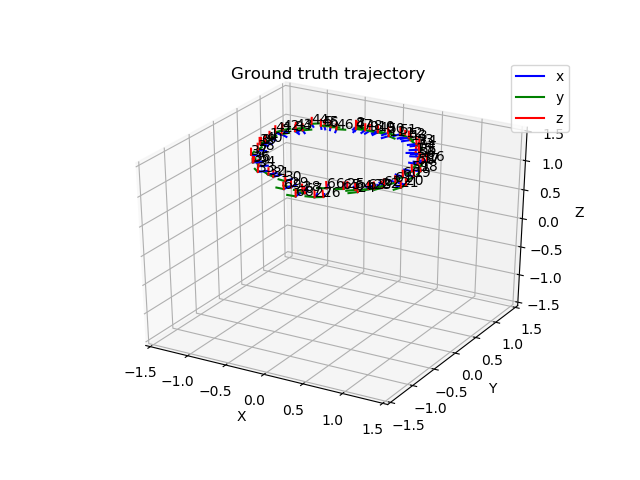
\includegraphics[width=80mm]{../2018-UAV-Registration/quad/basic-reg-saves/rtrj_gt.png}
  \caption{Ground truth from Vicon}
  \end{subfigure}
  \\
  \begin{subfigure}[t]{0.5\textwidth}
  \centering
    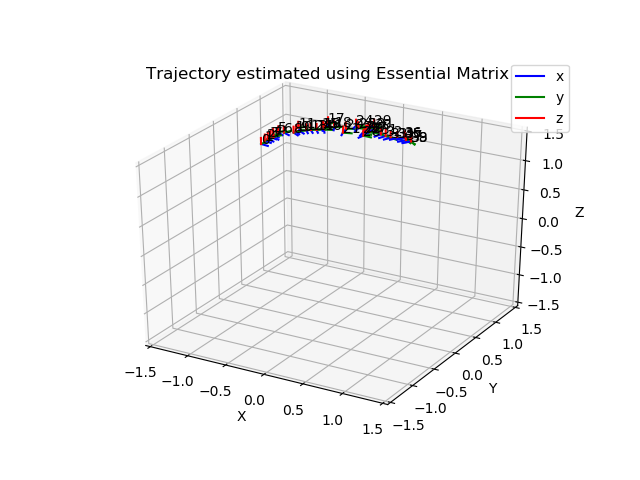
\includegraphics[width=80mm]{../2018-UAV-Registration/quad/basic-reg-saves/rtrj_rgb.png}
  \caption{Estimated trajectory for Essential Matrix method, start at origin}
  \end{subfigure}%
  ~
  \begin{subfigure}[t]{0.5\textwidth}
  \centering
    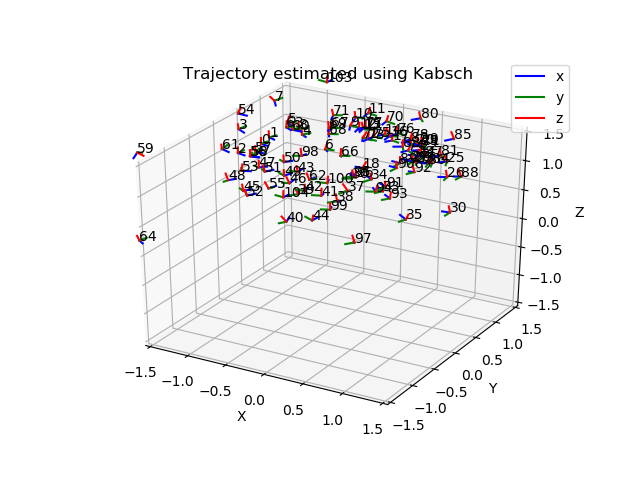
\includegraphics[width=80mm]{../2018-UAV-Registration/quad/basic-reg-saves/rtrj_d.png}
  \caption{Estimated trajectory for Kabsch method, start at origin}
  \end{subfigure}
  \\
  \begin{subfigure}[t]{0.5\textwidth}
  \centering
    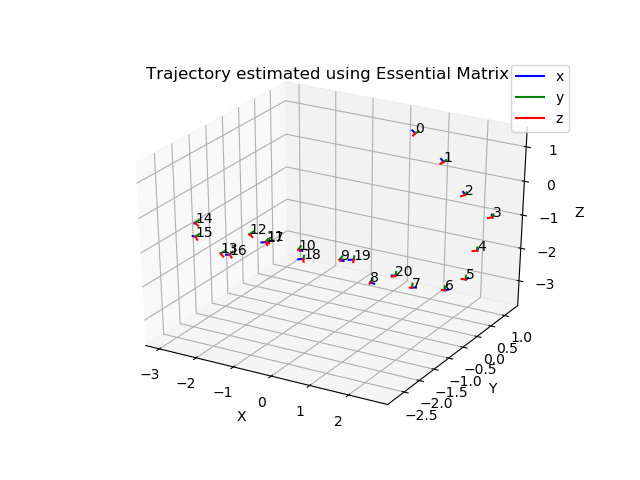
\includegraphics[width=80mm]{../2018-UAV-Registration/quad/basic-reg-saves/rtrj_rgb_start.png}
  \caption{Estimated trajectory for Essential Matrix method, start at ground truth}
  \end{subfigure}%
  ~
  \begin{subfigure}[t]{0.5\textwidth}
  \centering
    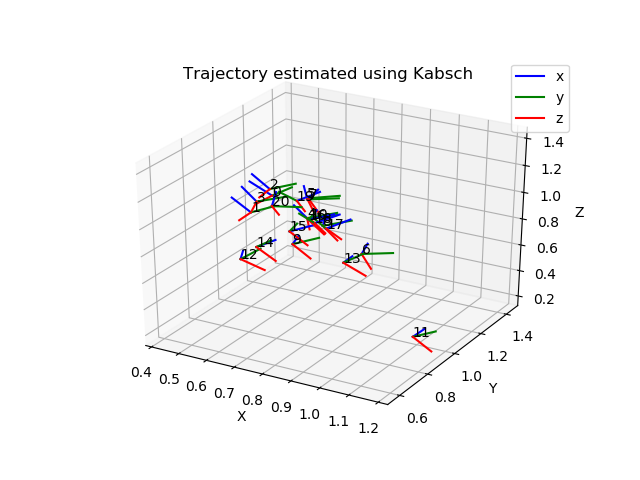
\includegraphics[width=80mm]{../2018-UAV-Registration/quad/basic-reg-saves/rtrj_d_start.png}
  \caption{Estimated trajectory for Kabsch method, start at ground truth}
  \end{subfigure}
  \caption{Trajectory visualizations for second quad dataset}
  \label{f: quad2 trj}
\end{figure}

\begin{figure}[h]
  \centering
  \begin{subfigure}[t]{\textwidth}
  \centering
  \includegraphics[width=120mm]{../2018-UAV-Registration/quad/matches/1533791885.82_essential.png}
  \caption{Points used for Essential Matrix}
  \end{subfigure}%
  \\
  \begin{subfigure}[t]{\textwidth}
  \centering
  \includegraphics[width=120mm]{../2018-UAV-Registration/quad/matches/1533791885.82_kabsch.png}
  \caption{Points used for Kabsch}
  \end{subfigure}%
  \caption{Matches after RANSAC (inliers) between two frames}
  \label{f: matches}
\end{figure}



% \begin{figure}[p]
%   \centering
%   \begin{subfigure}[t]{\textwidth}
%   \centering
%   \includegraphics[width=140mm]{../2018-UAV-Registration/quad/PCs/1533792217.77_PQ.png}
%   \caption{Point clouds used for one frame of Kabsch}
%   \end{subfigure}
%   \\
%   \begin{subfigure}[t]{0.5\textwidth}
%   \centering
%   \includegraphics[width=60mm]{../2018-UAV-Registration/quad/PCs/1533792217.77_PQ-aligned.png}
%   \caption{Point clouds used for one frame of Kabsch, first point cloud P aligned with second point cloud Q using found rotation and translation}
%   \end{subfigure}%
%   ~
%     \begin{subfigure}[t]{0.5\textwidth}
%   \centering
%   \includegraphics[width=60mm]{../2018-UAV-Registration/quad/PCs/1533792217.77_PQ-aligned-no.png}
%   \caption{Point clouds used for one frame of Kabsch, first point cloud P aligned with second point cloud Q using found rotation with no translation}
%   \end{subfigure}
%   \caption{Kabsch point clouds for quadcopter. Currently using scaling factor = 1 which is too big.}
%   \label{f: Kabsch quad good}
% \end{figure}

% \begin{figure}[p]
%   \centering
%   \begin{subfigure}[t]{\textwidth}
%   \centering
%   \includegraphics[width=140mm]{../2018-UAV-Registration/quad/PCs/1533792221.1_PQ.png}
%   \caption{Point clouds used for one frame of Kabsch}
%   \end{subfigure}
%   \\
%   \begin{subfigure}[t]{0.5\textwidth}
%   \centering
%   \includegraphics[width=60mm]{../2018-UAV-Registration/quad/PCs/1533792221.1_PQ-aligned.png}
%   \caption{Point clouds used for one frame of Kabsch, first point cloud P aligned with second point cloud Q using found rotation and translation}
%   \end{subfigure}%
%   ~
%     \begin{subfigure}[t]{0.5\textwidth}
%   \centering
%   \includegraphics[width=60mm]{../2018-UAV-Registration/quad/PCs/1533792221.1_PQ-aligned-no.png}
%   \caption{Point clouds used for one frame of Kabsch, first point cloud P aligned with second point cloud Q using found rotation with no translation}
%   \end{subfigure}
%   \caption{Kabsch point clouds for quadcopter. Currently using scaling factor = 1 which is too big.}
%   \label{f: Kabsch quad bad}
% \end{figure}



\bibliographystyle{abbrvnat}
\bibliography{../Report/ENGN4217}

\end{document}